\documentclass[twoside]{book}

% Packages required by doxygen
\usepackage{fixltx2e}
\usepackage{calc}
\usepackage{doxygen}
\usepackage[export]{adjustbox} % also loads graphicx
\usepackage{graphicx}
\usepackage[utf8]{inputenc}
\usepackage{makeidx}
\usepackage{multicol}
\usepackage{multirow}
\PassOptionsToPackage{warn}{textcomp}
\usepackage{textcomp}
\usepackage[nointegrals]{wasysym}
\usepackage[table]{xcolor}

% Font selection
\usepackage[T1]{fontenc}
\usepackage[scaled=.90]{helvet}
\usepackage{courier}
\usepackage{amssymb}
\usepackage{sectsty}
\renewcommand{\familydefault}{\sfdefault}
\allsectionsfont{%
  \fontseries{bc}\selectfont%
  \color{darkgray}%
}
\renewcommand{\DoxyLabelFont}{%
  \fontseries{bc}\selectfont%
  \color{darkgray}%
}
\newcommand{\+}{\discretionary{\mbox{\scriptsize$\hookleftarrow$}}{}{}}

% Page & text layout
\usepackage{geometry}
\geometry{%
  a4paper,%
  top=2.5cm,%
  bottom=2.5cm,%
  left=2.5cm,%
  right=2.5cm%
}
\tolerance=750
\hfuzz=15pt
\hbadness=750
\setlength{\emergencystretch}{15pt}
\setlength{\parindent}{0cm}
\setlength{\parskip}{3ex plus 2ex minus 2ex}
\makeatletter
\renewcommand{\paragraph}{%
  \@startsection{paragraph}{4}{0ex}{-1.0ex}{1.0ex}{%
    \normalfont\normalsize\bfseries\SS@parafont%
  }%
}
\renewcommand{\subparagraph}{%
  \@startsection{subparagraph}{5}{0ex}{-1.0ex}{1.0ex}{%
    \normalfont\normalsize\bfseries\SS@subparafont%
  }%
}
\makeatother

% Headers & footers
\usepackage{fancyhdr}
\pagestyle{fancyplain}
\fancyhead[LE]{\fancyplain{}{\bfseries\thepage}}
\fancyhead[CE]{\fancyplain{}{}}
\fancyhead[RE]{\fancyplain{}{\bfseries\leftmark}}
\fancyhead[LO]{\fancyplain{}{\bfseries\rightmark}}
\fancyhead[CO]{\fancyplain{}{}}
\fancyhead[RO]{\fancyplain{}{\bfseries\thepage}}
\fancyfoot[LE]{\fancyplain{}{}}
\fancyfoot[CE]{\fancyplain{}{}}
\fancyfoot[RE]{\fancyplain{}{\bfseries\scriptsize Generated by Doxygen }}
\fancyfoot[LO]{\fancyplain{}{\bfseries\scriptsize Generated by Doxygen }}
\fancyfoot[CO]{\fancyplain{}{}}
\fancyfoot[RO]{\fancyplain{}{}}
\renewcommand{\footrulewidth}{0.4pt}
\renewcommand{\chaptermark}[1]{%
  \markboth{#1}{}%
}
\renewcommand{\sectionmark}[1]{%
  \markright{\thesection\ #1}%
}

% Indices & bibliography
\usepackage{natbib}
\usepackage[titles]{tocloft}
\setcounter{tocdepth}{3}
\setcounter{secnumdepth}{5}
\makeindex

% Hyperlinks (required, but should be loaded last)
\usepackage{ifpdf}
\ifpdf
  \usepackage[pdftex,pagebackref=true]{hyperref}
\else
  \usepackage[ps2pdf,pagebackref=true]{hyperref}
\fi
\hypersetup{%
  colorlinks=true,%
  linkcolor=blue,%
  citecolor=blue,%
  unicode%
}

% Custom commands
\newcommand{\clearemptydoublepage}{%
  \newpage{\pagestyle{empty}\cleardoublepage}%
}

\usepackage{caption}
\captionsetup{labelsep=space,justification=centering,font={bf},singlelinecheck=off,skip=4pt,position=top}

%===== C O N T E N T S =====

\begin{document}

% Titlepage & ToC
\hypersetup{pageanchor=false,
             bookmarksnumbered=true,
             pdfencoding=unicode
            }
\pagenumbering{alph}
\begin{titlepage}
\vspace*{7cm}
\begin{center}%
{\Large libgai }\\
\vspace*{1cm}
{\large Generated by Doxygen 1.8.13}\\
\end{center}
\end{titlepage}
\clearemptydoublepage
\pagenumbering{roman}
\tableofcontents
\clearemptydoublepage
\pagenumbering{arabic}
\hypersetup{pageanchor=true}

%--- Begin generated contents ---
\chapter{libgai documentation}
\label{index}\hypertarget{index}{}\hypertarget{index_intro_sec}{}\section{Introduction}\label{index_intro_sec}
A list of all api\textquotesingle{}s currently available. \begin{DoxyNote}{Note}
None of these are actually done yet. They are working but do not support all features!
\end{DoxyNote}
\tabulinesep=1mm
\begin{longtabu} spread 0pt [c]{*{2}{|X[-1]}|}
\hline
\rowcolor{\tableheadbgcolor}\textbf{ filename }&\textbf{ description  }\\\cline{1-2}
\endfirsthead
\hline
\endfoot
\hline
\rowcolor{\tableheadbgcolor}\textbf{ filename }&\textbf{ description  }\\\cline{1-2}
\endhead
\hyperlink{gai__hotreload_8h}{gai\+\_\+hotreload.\+h} &Tracks when a file change happened to a file ( For windows it only check for filetime write changes. So it will trigger an event when you save the file or replace it with another ) \\\cline{1-2}
\hyperlink{gai__xwindow_8h}{gai\+\_\+xwindow.\+h} &Requests a window for all currently supported platforms. \\\cline{1-2}
\end{longtabu}

\chapter{Class Index}
\section{Class List}
Here are the classes, structs, unions and interfaces with brief descriptions\+:\begin{DoxyCompactList}
\item\contentsline{section}{\hyperlink{structgaihr__file}{gaihr\+\_\+file} }{\pageref{structgaihr__file}}{}
\item\contentsline{section}{\hyperlink{uniongaihr__file_8platform}{gaihr\+\_\+file.\+platform} }{\pageref{uniongaihr__file_8platform}}{}
\item\contentsline{section}{\hyperlink{structgaihr__file_8platform_8win32}{gaihr\+\_\+file.\+platform.\+win32} }{\pageref{structgaihr__file_8platform_8win32}}{}
\item\contentsline{section}{\hyperlink{structgaihr__filetime}{gaihr\+\_\+filetime} }{\pageref{structgaihr__filetime}}{}
\item\contentsline{section}{\hyperlink{structgaixw__context}{gaixw\+\_\+context} }{\pageref{structgaixw__context}}{}
\item\contentsline{section}{\hyperlink{structgaixw__context_8frametime}{gaixw\+\_\+context.\+frametime} }{\pageref{structgaixw__context_8frametime}}{}
\item\contentsline{section}{\hyperlink{structgaixw__context_8info}{gaixw\+\_\+context.\+info} }{\pageref{structgaixw__context_8info}}{}
\item\contentsline{section}{\hyperlink{structgaixw__context_8input}{gaixw\+\_\+context.\+input} }{\pageref{structgaixw__context_8input}}{}
\item\contentsline{section}{\hyperlink{uniongaixw__context_8platform}{gaixw\+\_\+context.\+platform} }{\pageref{uniongaixw__context_8platform}}{}
\item\contentsline{section}{\hyperlink{structgaixw__context_8platform_8linux}{gaixw\+\_\+context.\+platform.\+linux} }{\pageref{structgaixw__context_8platform_8linux}}{}
\item\contentsline{section}{\hyperlink{structgaixw__context_8platform_8win32}{gaixw\+\_\+context.\+platform.\+win32} }{\pageref{structgaixw__context_8platform_8win32}}{}
\item\contentsline{section}{\hyperlink{structgaixw__context_8renderer}{gaixw\+\_\+context.\+renderer} }{\pageref{structgaixw__context_8renderer}}{}
\item\contentsline{section}{\hyperlink{uniongaixw__context_8renderer_8info}{gaixw\+\_\+context.\+renderer.\+info} }{\pageref{uniongaixw__context_8renderer_8info}}{}
\item\contentsline{section}{\hyperlink{structgaixw__context_8renderer_8info_8opengl}{gaixw\+\_\+context.\+renderer.\+info.\+opengl} }{\pageref{structgaixw__context_8renderer_8info_8opengl}}{}
\item\contentsline{section}{\hyperlink{structgaixw__deinit__callback}{gaixw\+\_\+deinit\+\_\+callback} }{\pageref{structgaixw__deinit__callback}}{}
\end{DoxyCompactList}

\chapter{File Index}
\section{File List}
Here is a list of all documented files with brief descriptions\+:\begin{DoxyCompactList}
\item\contentsline{section}{{\bfseries doxygen.\+h} }{\pageref{doxygen_8h}}{}
\item\contentsline{section}{\hyperlink{gai_8h}{gai.\+h} \\*Designed as a cross platform single include header file for the most necessary features (window, dynamic array, qsort, network) }{\pageref{gai_8h}}{}
\item\contentsline{section}{{\bfseries gai\+\_\+engine.\+h} }{\pageref{gai__engine_8h}}{}
\end{DoxyCompactList}

\chapter{Class Documentation}
\hypertarget{structgaihr__file}{}\section{gaihr\+\_\+file Struct Reference}
\label{structgaihr__file}\index{gaihr\+\_\+file@{gaihr\+\_\+file}}


{\ttfamily \#include $<$gai\+\_\+hotreload.\+h$>$}

\subsection*{Public Attributes}
\begin{DoxyCompactItemize}
\item 
void $\ast$ \hyperlink{structgaihr__file_a06bf963cb9c08e69fcc6c4bb3140a2b8}{userdata}
\item 
gaihr\+\_\+callback $\ast$ \hyperlink{structgaihr__file_a9ac45c0142ff1eaf591b870e163d7f31}{callback}
\item 
\begin{tabbing}
xx\=xx\=xx\=xx\=xx\=xx\=xx\=xx\=xx\=\kill
union \{\\
\mbox{\Hypertarget{structgaihr__file_a47f5c92e431941d1123bffe57ab5e9ea}\label{structgaihr__file_a47f5c92e431941d1123bffe57ab5e9ea}} 
\>struct \{\\
\mbox{\Hypertarget{structgaihr__file_1_1_0D0_1_1_0D1_abd67073f9e6f24b8e2b2f04830dcf26a}\label{structgaihr__file_1_1_0D0_1_1_0D1_abd67073f9e6f24b8e2b2f04830dcf26a}} 
HANDLE {\bfseries mutex}\\
\mbox{\Hypertarget{structgaihr__file_1_1_0D0_1_1_0D1_a2b78d69604475cbeaa4fe29423b29523}\label{structgaihr__file_1_1_0D0_1_1_0D1_a2b78d69604475cbeaa4fe29423b29523}} 
HANDLE {\bfseries event}\\
\>\} {\bfseries win32}\\
\} \hyperlink{structgaihr__file_a4fa6fa162b2b39b5c54c260271ad6169}{platform}\\

\end{tabbing}\item 
\hyperlink{structgaihr__filetime}{gaihr\+\_\+filetime} \hyperlink{structgaihr__file_a38b2bc43116a1fd59715ca1714d80462}{last\+\_\+write\+\_\+time}
\item 
const char $\ast$ \hyperlink{structgaihr__file_a26ea2bbf62231c3cae2317ca217f8166}{filename}
\item 
gaihr\+\_\+flags \hyperlink{structgaihr__file_ab6eef82d50a8a51d161de3ab7ad98ee9}{flags}
\end{DoxyCompactItemize}


\subsection{Detailed Description}
\begin{DoxyRefDesc}{Todo}
\item[\hyperlink{todo__todo000001}{Todo}]Think about a way of easily support other platforms. \end{DoxyRefDesc}


\subsection{Member Data Documentation}
\mbox{\Hypertarget{structgaihr__file_a9ac45c0142ff1eaf591b870e163d7f31}\label{structgaihr__file_a9ac45c0142ff1eaf591b870e163d7f31}} 
\index{gaihr\+\_\+file@{gaihr\+\_\+file}!callback@{callback}}
\index{callback@{callback}!gaihr\+\_\+file@{gaihr\+\_\+file}}
\subsubsection{\texorpdfstring{callback}{callback}}
{\footnotesize\ttfamily gaihr\+\_\+callback$\ast$ gaihr\+\_\+file\+::callback}

Callback to the function when an event happens. See gaihr\+\_\+callback() \mbox{\Hypertarget{structgaihr__file_a26ea2bbf62231c3cae2317ca217f8166}\label{structgaihr__file_a26ea2bbf62231c3cae2317ca217f8166}} 
\index{gaihr\+\_\+file@{gaihr\+\_\+file}!filename@{filename}}
\index{filename@{filename}!gaihr\+\_\+file@{gaihr\+\_\+file}}
\subsubsection{\texorpdfstring{filename}{filename}}
{\footnotesize\ttfamily const char$\ast$ gaihr\+\_\+file\+::filename}

File to check for changes. \mbox{\Hypertarget{structgaihr__file_ab6eef82d50a8a51d161de3ab7ad98ee9}\label{structgaihr__file_ab6eef82d50a8a51d161de3ab7ad98ee9}} 
\index{gaihr\+\_\+file@{gaihr\+\_\+file}!flags@{flags}}
\index{flags@{flags}!gaihr\+\_\+file@{gaihr\+\_\+file}}
\subsubsection{\texorpdfstring{flags}{flags}}
{\footnotesize\ttfamily gaihr\+\_\+flags gaihr\+\_\+file\+::flags}

Flags to specify event handling and callback behaviour. \mbox{\Hypertarget{structgaihr__file_a38b2bc43116a1fd59715ca1714d80462}\label{structgaihr__file_a38b2bc43116a1fd59715ca1714d80462}} 
\index{gaihr\+\_\+file@{gaihr\+\_\+file}!last\+\_\+write\+\_\+time@{last\+\_\+write\+\_\+time}}
\index{last\+\_\+write\+\_\+time@{last\+\_\+write\+\_\+time}!gaihr\+\_\+file@{gaihr\+\_\+file}}
\subsubsection{\texorpdfstring{last\+\_\+write\+\_\+time}{last\_write\_time}}
{\footnotesize\ttfamily \hyperlink{structgaihr__filetime}{gaihr\+\_\+filetime} gaihr\+\_\+file\+::last\+\_\+write\+\_\+time}

Filetime structure. \mbox{\Hypertarget{structgaihr__file_a4fa6fa162b2b39b5c54c260271ad6169}\label{structgaihr__file_a4fa6fa162b2b39b5c54c260271ad6169}} 
\index{gaihr\+\_\+file@{gaihr\+\_\+file}!platform@{platform}}
\index{platform@{platform}!gaihr\+\_\+file@{gaihr\+\_\+file}}
\subsubsection{\texorpdfstring{platform}{platform}}
{\footnotesize\ttfamily union \{ ... \}   gaihr\+\_\+file\+::platform}

Platform specfic structure for semaphore or mutex handles. \mbox{\Hypertarget{structgaihr__file_a06bf963cb9c08e69fcc6c4bb3140a2b8}\label{structgaihr__file_a06bf963cb9c08e69fcc6c4bb3140a2b8}} 
\index{gaihr\+\_\+file@{gaihr\+\_\+file}!userdata@{userdata}}
\index{userdata@{userdata}!gaihr\+\_\+file@{gaihr\+\_\+file}}
\subsubsection{\texorpdfstring{userdata}{userdata}}
{\footnotesize\ttfamily void$\ast$ gaihr\+\_\+file\+::userdata}

User passed data. 

The documentation for this struct was generated from the following file\+:\begin{DoxyCompactItemize}
\item 
gai\+\_\+hotreload.\+h\end{DoxyCompactItemize}

\hypertarget{structgaihr__platform}{}\section{gaihr\+\_\+platform Struct Reference}
\label{structgaihr__platform}\index{gaihr\+\_\+platform@{gaihr\+\_\+platform}}


Platform specific hotreload layer with mutex and event handles. Should not be used outside of this file!  




{\ttfamily \#include $<$gai\+\_\+hotreload.\+h$>$}

\subsection*{Public Attributes}
\begin{DoxyCompactItemize}
\item 
H\+A\+N\+D\+LE \hyperlink{structgaihr__platform_a4502c637972f49cbb803c93975fe45f4}{mutex}
\item 
H\+A\+N\+D\+LE \hyperlink{structgaihr__platform_a702622bb26128f36b2c27c8ffdb1b7a0}{event}
\item 
F\+I\+L\+E\+T\+I\+ME \hyperlink{structgaihr__platform_a6be2e4d6d98523e09c04a19b20d04cd1}{last\+\_\+write\+\_\+time}
\end{DoxyCompactItemize}


\subsection{Detailed Description}
Platform specific hotreload layer with mutex and event handles. Should not be used outside of this file! 

This struct will vary on different platforms. T\+O\+DO\+: Add support for multiple platforms! 

\subsection{Member Data Documentation}
\mbox{\Hypertarget{structgaihr__platform_a702622bb26128f36b2c27c8ffdb1b7a0}\label{structgaihr__platform_a702622bb26128f36b2c27c8ffdb1b7a0}} 
\index{gaihr\+\_\+platform@{gaihr\+\_\+platform}!event@{event}}
\index{event@{event}!gaihr\+\_\+platform@{gaihr\+\_\+platform}}
\subsubsection{\texorpdfstring{event}{event}}
{\footnotesize\ttfamily H\+A\+N\+D\+LE gaihr\+\_\+platform\+::event}

Handle to a windows event \mbox{\Hypertarget{structgaihr__platform_a6be2e4d6d98523e09c04a19b20d04cd1}\label{structgaihr__platform_a6be2e4d6d98523e09c04a19b20d04cd1}} 
\index{gaihr\+\_\+platform@{gaihr\+\_\+platform}!last\+\_\+write\+\_\+time@{last\+\_\+write\+\_\+time}}
\index{last\+\_\+write\+\_\+time@{last\+\_\+write\+\_\+time}!gaihr\+\_\+platform@{gaihr\+\_\+platform}}
\subsubsection{\texorpdfstring{last\+\_\+write\+\_\+time}{last\_write\_time}}
{\footnotesize\ttfamily F\+I\+L\+E\+T\+I\+ME gaihr\+\_\+platform\+::last\+\_\+write\+\_\+time}

Timestamp of last change \mbox{\Hypertarget{structgaihr__platform_a4502c637972f49cbb803c93975fe45f4}\label{structgaihr__platform_a4502c637972f49cbb803c93975fe45f4}} 
\index{gaihr\+\_\+platform@{gaihr\+\_\+platform}!mutex@{mutex}}
\index{mutex@{mutex}!gaihr\+\_\+platform@{gaihr\+\_\+platform}}
\subsubsection{\texorpdfstring{mutex}{mutex}}
{\footnotesize\ttfamily H\+A\+N\+D\+LE gaihr\+\_\+platform\+::mutex}

Handle to a windows mutex 

The documentation for this struct was generated from the following file\+:\begin{DoxyCompactItemize}
\item 
\hyperlink{gai__hotreload_8h}{gai\+\_\+hotreload.\+h}\end{DoxyCompactItemize}

\chapter{File Documentation}
\hypertarget{gai__hotreload_8h}{}\section{gai\+\_\+hotreload.\+h File Reference}
\label{gai__hotreload_8h}\index{gai\+\_\+hotreload.\+h@{gai\+\_\+hotreload.\+h}}


Tracks when a file change happened to a file ( For windows it only check for filetime write changes. So it will trigger an event when you save the file or replace it with another )  


{\ttfamily \#include $<$windows.\+h$>$}\newline
{\ttfamily \#include $<$assert.\+h$>$}\newline
Include dependency graph for gai\+\_\+hotreload.\+h\+:\nopagebreak
\begin{figure}[H]
\begin{center}
\leavevmode
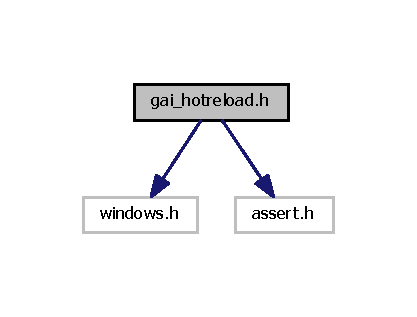
\includegraphics[width=200pt]{gai__hotreload_8h__incl}
\end{center}
\end{figure}
\subsection*{Classes}
\begin{DoxyCompactItemize}
\item 
union \hyperlink{gai__hotreload_8h_uniongaihr__filetime}{gaihr\+\_\+filetime}
\item 
union \hyperlink{gai__hotreload_8h_uniongaihr__platform}{gaihr\+\_\+platform}
\item 
struct \hyperlink{gai__hotreload_8h_structgaihr__platform_1_1gaihr__platform__win32}{gaihr\+\_\+platform\+::gaihr\+\_\+platform\+\_\+win32}
\item 
struct \hyperlink{gai__hotreload_8h_structgaihr__platform_1_1gaihr__platform__linux}{gaihr\+\_\+platform\+::gaihr\+\_\+platform\+\_\+linux}
\item 
struct \hyperlink{gai__hotreload_8h_structgaihr__file}{gaihr\+\_\+file}
\item 
struct \hyperlink{gai__hotreload_8h_structgaihr__filetime_8parts}{gaihr\+\_\+filetime.\+parts}
\end{DoxyCompactItemize}
\subsection*{Macros}
\begin{DoxyCompactItemize}
\item 
\#define \hyperlink{gai__hotreload_8h_a36b03891b740d035afdd1f32e15c91ad}{G\+A\+I\+H\+R\+\_\+\+W\+A\+I\+T\+\_\+\+I\+N\+F\+I\+N\+I\+TE}~-\/1
\item 
\#define \hyperlink{gai__hotreload_8h_a7385b7149ef022fa38140e2b2a540502}{G\+A\+I\+H\+R\+\_\+\+T\+H\+R\+E\+A\+D\+\_\+\+T\+I\+M\+E\+O\+UT}~1000
\item 
\#define \hyperlink{gai__hotreload_8h_ac26b515249679c1f9036430164867ba0}{G\+A\+I\+H\+R\+\_\+\+F\+I\+L\+E\+\_\+\+L\+I\+M\+IT}~64
\item 
\mbox{\Hypertarget{gai__hotreload_8h_a32983003a4e816a8350f01cb22d1b01b}\label{gai__hotreload_8h_a32983003a4e816a8350f01cb22d1b01b}} 
\#define \hyperlink{gai__hotreload_8h_a32983003a4e816a8350f01cb22d1b01b}{G\+A\+I\+H\+R\+\_\+\+A\+PI}~extern
\begin{DoxyCompactList}\small\item\em Define {\bfseries G\+A\+I\+H\+R\+\_\+\+S\+T\+A\+T\+IC} if you want to make functions {\bfseries static} instead of {\bfseries extern} \end{DoxyCompactList}\item 
\#define \hyperlink{gai__hotreload_8h_a11e965cbb3e2af8ed1888b0c6b2777da}{G\+A\+I\+H\+R\+\_\+\+A\+S\+S\+E\+RT}(cond)~assert(cond)
\begin{DoxyCompactList}\small\item\em Define {\bfseries G\+A\+I\+H\+R\+\_\+\+A\+S\+S\+E\+RT} before including this file to {\bfseries disable} assertions. \end{DoxyCompactList}\item 
\#define \hyperlink{gai__hotreload_8h_a6f8c5bfe220445bbbb8e1c9ef176838a}{G\+A\+I\+H\+R\+\_\+\+C\+A\+L\+L\+B\+A\+CK}(name)~void name(\hyperlink{gai__hotreload_8h_structgaihr__file}{gaihr\+\_\+file} $\ast$file)
\begin{DoxyCompactList}\small\item\em Callback function macro which will generate a function as specified by \hyperlink{gai__hotreload_8h_a8026f464cf8636b763b6f03798d40800}{gaihr\+\_\+callback}. \end{DoxyCompactList}\end{DoxyCompactItemize}
\subsection*{Typedefs}
\begin{DoxyCompactItemize}
\item 
\mbox{\Hypertarget{gai__hotreload_8h_a8026f464cf8636b763b6f03798d40800}\label{gai__hotreload_8h_a8026f464cf8636b763b6f03798d40800}} 
typedef void \hyperlink{gai__hotreload_8h_a8026f464cf8636b763b6f03798d40800}{gaihr\+\_\+callback}(\hyperlink{gai__hotreload_8h_structgaihr__file}{gaihr\+\_\+file} $\ast$file)
\begin{DoxyCompactList}\small\item\em Callback function which will be called when an event was fired See \hyperlink{gai__hotreload_8h_a6f8c5bfe220445bbbb8e1c9ef176838a}{G\+A\+I\+H\+R\+\_\+\+C\+A\+L\+L\+B\+A\+CK}. \end{DoxyCompactList}\end{DoxyCompactItemize}
\subsection*{Enumerations}
\begin{DoxyCompactItemize}
\item 
enum \hyperlink{gai__hotreload_8h_aaebb069b6896f065efd75640e0e4150b}{gaihr\+\_\+flags} \{ \hyperlink{gai__hotreload_8h_aaebb069b6896f065efd75640e0e4150ba6c207a28fdce6637b4aa1e70e64c3e94}{gaihr\+\_\+\+Flags\+None} = 0x0, 
\hyperlink{gai__hotreload_8h_aaebb069b6896f065efd75640e0e4150ba158375938f45efe930ee7416d19e5a6c}{gaihr\+\_\+\+Flags\+Dont\+Handle\+Event} = 0x1, 
\hyperlink{gai__hotreload_8h_aaebb069b6896f065efd75640e0e4150babfc4c1c7557333f4e2cddf40cacefc7a}{gaihr\+\_\+\+Flags\+Dont\+Reset\+Event} = 0x2, 
\hyperlink{gai__hotreload_8h_aaebb069b6896f065efd75640e0e4150baee50ce1492a508e5605592106fa00bd5}{gaihr\+\_\+\+Flags\+Skip\+Initial\+Change} = 0x4
 \}\begin{DoxyCompactList}\small\item\em This flags specify how the event and callback function will be handled. \end{DoxyCompactList}
\end{DoxyCompactItemize}
\subsection*{Functions}
\begin{DoxyCompactItemize}
\item 
\hyperlink{gai__hotreload_8h_a32983003a4e816a8350f01cb22d1b01b}{G\+A\+I\+H\+R\+\_\+\+A\+PI} unsigned int \hyperlink{gai__hotreload_8h_ad83d8f6170f0404fb72803d012ac9f6a}{gaihr\+\_\+\+Track} (\hyperlink{gai__hotreload_8h_structgaihr__file}{gaihr\+\_\+file} $\ast$file, const char $\ast$filename, \hyperlink{gai__hotreload_8h_a8026f464cf8636b763b6f03798d40800}{gaihr\+\_\+callback} $\ast$callback=0, void $\ast$userdata=0, \hyperlink{gai__hotreload_8h_aaebb069b6896f065efd75640e0e4150b}{gaihr\+\_\+flags} flags=\hyperlink{gai__hotreload_8h_aaebb069b6896f065efd75640e0e4150ba6c207a28fdce6637b4aa1e70e64c3e94}{gaihr\+\_\+\+Flags\+None})
\begin{DoxyCompactList}\small\item\em Adds a file to a worker thread, which internally tracks if the given file was modified. If so it will fire an event which will result in a function call to the callback function or handled differently depending on the specified flags. \end{DoxyCompactList}\item 
\hyperlink{gai__hotreload_8h_a32983003a4e816a8350f01cb22d1b01b}{G\+A\+I\+H\+R\+\_\+\+A\+PI} unsigned int \hyperlink{gai__hotreload_8h_a288369c901929574624b267de90007cd}{gaihr\+\_\+\+Untrack} (\hyperlink{gai__hotreload_8h_structgaihr__file}{gaihr\+\_\+file} $\ast$file)
\begin{DoxyCompactList}\small\item\em Removes a file from the worker thread. \end{DoxyCompactList}\item 
\hyperlink{gai__hotreload_8h_a32983003a4e816a8350f01cb22d1b01b}{G\+A\+I\+H\+R\+\_\+\+A\+PI} void \hyperlink{gai__hotreload_8h_a79d4ca28cdaae457474d55a0a21dd326}{gaihr\+\_\+\+Wait\+For\+Event} (\hyperlink{gai__hotreload_8h_structgaihr__file}{gaihr\+\_\+file} $\ast$file)
\begin{DoxyCompactList}\small\item\em Grabs a mutex for the specified \hyperlink{gai__hotreload_8h_structgaihr__file}{gaihr\+\_\+file} handle and waits for an event. If a callback function is specifed and an event happend the callback function will be called. \end{DoxyCompactList}\item 
\hyperlink{gai__hotreload_8h_a32983003a4e816a8350f01cb22d1b01b}{G\+A\+I\+H\+R\+\_\+\+A\+PI} unsigned int \hyperlink{gai__hotreload_8h_a52aa011dc92eb63b9d5fc7993042eb3f}{\+\_\+gaihr\+\_\+\+Begin\+Ticket\+Mutex} (\hyperlink{gai__hotreload_8h_structgaihr__file}{gaihr\+\_\+file} $\ast$file, int timeout=\hyperlink{gai__hotreload_8h_a36b03891b740d035afdd1f32e15c91ad}{G\+A\+I\+H\+R\+\_\+\+W\+A\+I\+T\+\_\+\+I\+N\+F\+I\+N\+I\+TE})
\begin{DoxyCompactList}\small\item\em Opens a mutex to access the data safely in a multi-\/threaded way. \end{DoxyCompactList}\item 
\hyperlink{gai__hotreload_8h_a32983003a4e816a8350f01cb22d1b01b}{G\+A\+I\+H\+R\+\_\+\+A\+PI} void \hyperlink{gai__hotreload_8h_ae6e501372d35a3645332dadb8f612e3c}{\+\_\+gaihr\+\_\+\+End\+Ticket\+Mutex} (\hyperlink{gai__hotreload_8h_structgaihr__file}{gaihr\+\_\+file} $\ast$file)
\begin{DoxyCompactList}\small\item\em Releases the previously opened mutex to allow other thread to use this mutex. \end{DoxyCompactList}\item 
\hyperlink{gai__hotreload_8h_a32983003a4e816a8350f01cb22d1b01b}{G\+A\+I\+H\+R\+\_\+\+A\+PI} void \hyperlink{gai__hotreload_8h_a465162f1865f5f804311c153c0995543}{\+\_\+gaihr\+\_\+\+Set\+Event} (\hyperlink{gai__hotreload_8h_structgaihr__file}{gaihr\+\_\+file} $\ast$file)
\begin{DoxyCompactList}\small\item\em Signals a file change to the user. \end{DoxyCompactList}\item 
\hyperlink{gai__hotreload_8h_a32983003a4e816a8350f01cb22d1b01b}{G\+A\+I\+H\+R\+\_\+\+A\+PI} void \hyperlink{gai__hotreload_8h_aba347f4afef1dd5f850142adf487fa26}{\+\_\+gaihr\+\_\+\+Reset\+Event} (\hyperlink{gai__hotreload_8h_structgaihr__file}{gaihr\+\_\+file} $\ast$file)
\begin{DoxyCompactList}\small\item\em Resets the previously set signal. \end{DoxyCompactList}\item 
\hyperlink{gai__hotreload_8h_a32983003a4e816a8350f01cb22d1b01b}{G\+A\+I\+H\+R\+\_\+\+A\+PI} int \hyperlink{gai__hotreload_8h_acee43647e5f69a31c40726d43bfe19e3}{\+\_\+gaihr\+\_\+\+Compare\+File\+Time} (\hyperlink{gai__hotreload_8h_uniongaihr__filetime}{gaihr\+\_\+filetime} $\ast$a, \hyperlink{gai__hotreload_8h_uniongaihr__filetime}{gaihr\+\_\+filetime} $\ast$b)
\begin{DoxyCompactList}\small\item\em Compare two gaihr\+\_\+filetimes to each other. \end{DoxyCompactList}\item 
\hyperlink{gai__hotreload_8h_a32983003a4e816a8350f01cb22d1b01b}{G\+A\+I\+H\+R\+\_\+\+A\+PI} void \hyperlink{gai__hotreload_8h_a7017705231a1470b0a03c14a9c28aa11}{\+\_\+gaihr\+\_\+\+Do\+Work} (\hyperlink{gai__hotreload_8h_structgaihr__file}{gaihr\+\_\+file} $\ast$$\ast$files)
\begin{DoxyCompactList}\small\item\em Loops through all files to track. \end{DoxyCompactList}\end{DoxyCompactItemize}
\subsection*{Variables}
\begin{DoxyCompactItemize}
\item 
\mbox{\Hypertarget{gai__hotreload_8h_affcc82be3377e9546e28872eda3caa5f}\label{gai__hotreload_8h_affcc82be3377e9546e28872eda3caa5f}} 
static \hyperlink{gai__hotreload_8h_structgaihr__file}{gaihr\+\_\+file} $\ast$ {\bfseries \+\_\+gaihr\+\_\+files} \mbox{[}\hyperlink{gai__hotreload_8h_ac26b515249679c1f9036430164867ba0}{G\+A\+I\+H\+R\+\_\+\+F\+I\+L\+E\+\_\+\+L\+I\+M\+IT}\mbox{]}
\end{DoxyCompactItemize}


\subsection{Detailed Description}
Tracks when a file change happened to a file ( For windows it only check for filetime write changes. So it will trigger an event when you save the file or replace it with another ) 

\begin{DoxyAttention}{Attention}
{\bfseries O\+N\+LY W\+I\+N\+D\+O\+WS IS S\+U\+P\+P\+O\+R\+T\+ED} ~\newline
 {\bfseries Linker dependencies\+: user32.\+lib}
\end{DoxyAttention}
\hypertarget{gai__hotreload_8h_gaihr_intro}{}\subsection{Introduction}\label{gai__hotreload_8h_gaihr_intro}
The tracking will take place on a seperate thread which will be started the first time you add a file via gaihr\+\_\+\+Track(...) call. You can specify different flags on how the event and callback function will be handled. See the \hyperlink{gai__hotreload_8h_aaebb069b6896f065efd75640e0e4150b}{gaihr\+\_\+flags} definition.

You can use this api to do hotreloading of dll\textquotesingle{}s or texture\textquotesingle{}s or just plain textfile\textquotesingle{}s.

Do this\+: \begin{DoxyVerb}#define GAIHR_IMPLEMENTATION
\end{DoxyVerb}


before you include this file in {\itshape one} C++ file to create the implementation.

\begin{DoxyNote}{Note}
{\bfseries All function prefixed with a underscore(\+\_\+) are internally used functions.} {\bfseries DO N\+OT use them if you are not 100\% sure what they do.}
\end{DoxyNote}
\hypertarget{gai__hotreload_8h_gaihr_code_example}{}\subsubsection{Example Code}\label{gai__hotreload_8h_gaihr_code_example}
A file with the name \char`\"{}testfile.\+txt\char`\"{} has to be in the directory of the executable. After running the executable you have to change the file\textquotesingle{}s content and save it or replace it with another file (same filename).


\begin{DoxyCodeInclude}
\textcolor{preprocessor}{#define GAIHR\_IMPLEMENTATION}
\textcolor{preprocessor}{#include "\hyperlink{gai__hotreload_8h}{gai\_hotreload.h}"}
\textcolor{preprocessor}{#include <stdio.h>}
\textcolor{preprocessor}{#include <stdlib.h>}

\textcolor{keyword}{volatile} \textcolor{keywordtype}{int} running = 1; \textcolor{comment}{// This will be changed by another thread!}

\hyperlink{gai__hotreload_8h_a6f8c5bfe220445bbbb8e1c9ef176838a}{GAIHR\_CALLBACK}(printFileContentAndStop)
\{
    \textcolor{keywordtype}{long} filesize = 0;
    \textcolor{keywordtype}{char} *filecontent = 0;
    \textcolor{keywordtype}{size\_t} result;
    running = 0;

    FILE *fp = fopen(file->filename, \textcolor{stringliteral}{"rb"});
    \textcolor{keywordflow}{if} (fp)
    \{
        fseek(fp , 0 , SEEK\_END);
        filesize = ftell(fp);
        rewind(fp);
        filecontent = (\textcolor{keywordtype}{char}*) malloc(filesize+1);
        \textcolor{keywordflow}{if} (!filecontent)
        \{
            fclose(fp);
            printf(\textcolor{stringliteral}{"malloc error\(\backslash\)n"});
            \textcolor{keywordflow}{return};
        \}

        result = fread(filecontent, 1, filesize, fp);
        \textcolor{keywordflow}{if} (result != filesize)
        \{
            fclose(fp);
            printf(\textcolor{stringliteral}{"file read failed\(\backslash\)n"});
            \textcolor{keywordflow}{return};
        \}
        filecontent[filesize] = 0;
        printf(\textcolor{stringliteral}{"%s changed!\(\backslash\)nnew file content:\(\backslash\)n%s\(\backslash\)n"}, file->filename, filecontent);
        free(filecontent);
        fclose(fp);
    \}
\}

\textcolor{keywordtype}{int} main(\textcolor{keywordtype}{int} argc, \textcolor{keywordtype}{char} **argv)
\{
    \hyperlink{gai__hotreload_8h_structgaihr__file}{gaihr\_file} MyFile = \{\};
    \hyperlink{gai__hotreload_8h_ad83d8f6170f0404fb72803d012ac9f6a}{gaihr\_Track}(&MyFile, \textcolor{stringliteral}{"testfile.txt"}, printFileContentAndStop, 0, 
      \hyperlink{gai__hotreload_8h_aaebb069b6896f065efd75640e0e4150baee50ce1492a508e5605592106fa00bd5}{gaihr\_FlagsSkipInitialChange});
    printf(\textcolor{stringliteral}{"Please change the file content or replace the file now...\(\backslash\)n"});
    \textcolor{keywordflow}{while} (running) \{Sleep(125);\}
    \textcolor{keywordflow}{return} 0;
\}
\end{DoxyCodeInclude}


\begin{DoxyAuthor}{Author}
Andreas Gaida 
\end{DoxyAuthor}
\begin{DoxyDate}{Date}
25.\+04.\+2017 
\end{DoxyDate}
\begin{DoxySeeAlso}{See also}
\href{https://github.com/LostinAllThatCode/libgai}{\tt https\+://github.\+com/\+Lostin\+All\+That\+Code/libgai} 
\end{DoxySeeAlso}


\subsection{Class Documentation}
\index{gaihr\+\_\+filetime@{gaihr\+\_\+filetime}}\label{uniongaihr__filetime}
\Hypertarget{gai__hotreload_8h_uniongaihr__filetime}
\subsubsection{union gaihr\+\_\+filetime}
\begin{DoxyFields}{Class Members}
\mbox{\Hypertarget{gai__hotreload_8h_a61446b486ff5dbcd62b9b83418d853ac}\label{gai__hotreload_8h_a61446b486ff5dbcd62b9b83418d853ac}} 
struct \hyperlink{gai__hotreload_8h_structgaihr__filetime_8parts}{gaihr\_filetime}&
parts&
This is here to easily cast windows F\+I\+L\+E\+T\+I\+ME structure to this one. \\
\hline

\mbox{\Hypertarget{gai__hotreload_8h_a17c62c2a56dc2b6f8ad20c3359562b2e}\label{gai__hotreload_8h_a17c62c2a56dc2b6f8ad20c3359562b2e}} 
unsigned long long&
time&
\\
\hline

\end{DoxyFields}
\index{gaihr\+\_\+platform@{gaihr\+\_\+platform}}\label{uniongaihr__platform}
\Hypertarget{gai__hotreload_8h_uniongaihr__platform}
\subsubsection{union gaihr\+\_\+platform}


Collaboration diagram for gaihr\+\_\+platform\+:\nopagebreak
\begin{figure}[H]
\begin{center}
\leavevmode
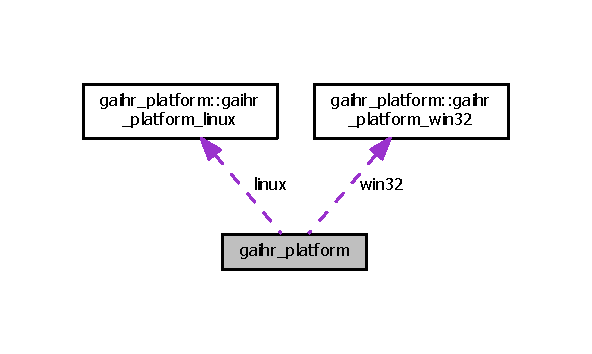
\includegraphics[width=284pt]{uniongaihr__platform__coll__graph}
\end{center}
\end{figure}
\begin{DoxyFields}{Class Members}
\mbox{\Hypertarget{gai__hotreload_8h_aff9109eeb79bcbee6ddf4eab05477a83}\label{gai__hotreload_8h_aff9109eeb79bcbee6ddf4eab05477a83}} 
struct \hyperlink{gai__hotreload_8h_structgaihr__platform_1_1gaihr__platform__linux}{gaihr\_platform\_linux}&
linux&
\\
\hline

\mbox{\Hypertarget{gai__hotreload_8h_ab100a9280dca047d4c625cbf6ea7e64c}\label{gai__hotreload_8h_ab100a9280dca047d4c625cbf6ea7e64c}} 
struct \hyperlink{gai__hotreload_8h_structgaihr__platform_1_1gaihr__platform__win32}{gaihr\_platform\_win32}&
win32&
\\
\hline

\end{DoxyFields}
\index{gaihr\+\_\+platform\+::gaihr\+\_\+platform\+\_\+win32@{gaihr\+\_\+platform\+::gaihr\+\_\+platform\+\_\+win32}}\label{structgaihr__platform_1_1gaihr__platform__win32}
\Hypertarget{gai__hotreload_8h_structgaihr__platform_1_1gaihr__platform__win32}
\subsubsection{struct gaihr\+\_\+platform\+:\+:gaihr\+\_\+platform\+\_\+win32}
\begin{DoxyFields}{Class Members}
\mbox{\Hypertarget{gai__hotreload_8h_aa9b31d30dfd3fa64e40b7cd771f98253}\label{gai__hotreload_8h_aa9b31d30dfd3fa64e40b7cd771f98253}} 
HANDLE&
event&
\\
\hline

\mbox{\Hypertarget{gai__hotreload_8h_ab17cd0ffa18b4ef60cd0d4736f0abc0a}\label{gai__hotreload_8h_ab17cd0ffa18b4ef60cd0d4736f0abc0a}} 
HANDLE&
mutex&
\\
\hline

\end{DoxyFields}
\index{gaihr\+\_\+platform\+::gaihr\+\_\+platform\+\_\+linux@{gaihr\+\_\+platform\+::gaihr\+\_\+platform\+\_\+linux}}\label{structgaihr__platform_1_1gaihr__platform__linux}
\Hypertarget{gai__hotreload_8h_structgaihr__platform_1_1gaihr__platform__linux}
\subsubsection{struct gaihr\+\_\+platform\+:\+:gaihr\+\_\+platform\+\_\+linux}
\begin{DoxyFields}{Class Members}
\mbox{\Hypertarget{gai__hotreload_8h_a50324e3fd2b5fdcfd27f1ae040656ac2}\label{gai__hotreload_8h_a50324e3fd2b5fdcfd27f1ae040656ac2}} 
void $\ast$&
event&
\\
\hline

\mbox{\Hypertarget{gai__hotreload_8h_a02af0c94ad547b2616feff49dcee343e}\label{gai__hotreload_8h_a02af0c94ad547b2616feff49dcee343e}} 
void $\ast$&
mutex&
\\
\hline

\end{DoxyFields}
\index{gaihr\+\_\+file@{gaihr\+\_\+file}}\label{structgaihr__file}
\Hypertarget{gai__hotreload_8h_structgaihr__file}
\subsubsection{struct gaihr\+\_\+file}
\begin{DoxyRefDesc}{Todo}
\item[\hyperlink{todo__todo000001}{Todo}]Think about a way of easily support other platforms. \end{DoxyRefDesc}
\begin{Desc}
\item[Examples\+: ]\par
\hyperlink{hotreload_0Cwin32_0Cmain_8cpp-example}{hotreload\textbackslash{}win32\textbackslash{}main.\+cpp}.\end{Desc}


Collaboration diagram for gaihr\+\_\+file\+:\nopagebreak
\begin{figure}[H]
\begin{center}
\leavevmode
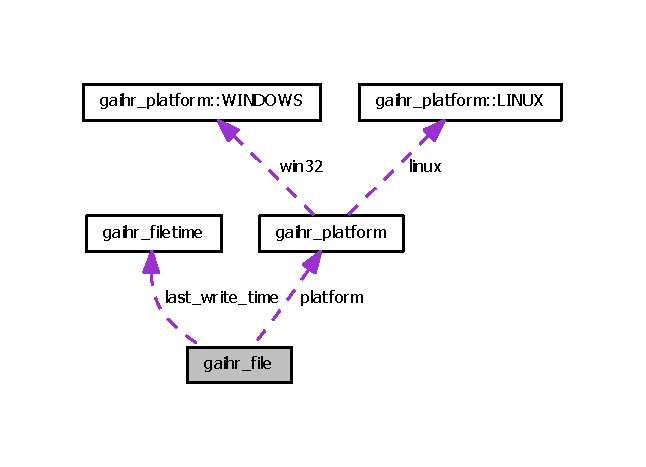
\includegraphics[width=299pt]{structgaihr__file__coll__graph}
\end{center}
\end{figure}
\begin{DoxyFields}{Class Members}
\mbox{\Hypertarget{gai__hotreload_8h_a9ac45c0142ff1eaf591b870e163d7f31}\label{gai__hotreload_8h_a9ac45c0142ff1eaf591b870e163d7f31}} 
\hyperlink{gai__hotreload_8h_a8026f464cf8636b763b6f03798d40800}{gaihr\_callback} $\ast$&
callback&
Callback to the function when an event happens. See \hyperlink{gai__hotreload_8h_a6f8c5bfe220445bbbb8e1c9ef176838a}{G\+A\+I\+H\+R\+\_\+\+C\+A\+L\+L\+B\+A\+CK} \\
\hline

\mbox{\Hypertarget{gai__hotreload_8h_a26ea2bbf62231c3cae2317ca217f8166}\label{gai__hotreload_8h_a26ea2bbf62231c3cae2317ca217f8166}} 
const char $\ast$&
filename&
File to check for changes. \\
\hline

\mbox{\Hypertarget{gai__hotreload_8h_ab6eef82d50a8a51d161de3ab7ad98ee9}\label{gai__hotreload_8h_ab6eef82d50a8a51d161de3ab7ad98ee9}} 
\hyperlink{gai__hotreload_8h_aaebb069b6896f065efd75640e0e4150b}{gaihr\_flags}&
flags&
Flags to specify event handling and callback behaviour. \\
\hline

\mbox{\Hypertarget{gai__hotreload_8h_a38b2bc43116a1fd59715ca1714d80462}\label{gai__hotreload_8h_a38b2bc43116a1fd59715ca1714d80462}} 
\hyperlink{gai__hotreload_8h_uniongaihr__filetime}{gaihr\_filetime}&
last\_write\_time&
Filetime structure. \\
\hline

\mbox{\Hypertarget{gai__hotreload_8h_a138044c270d5f0e83917ae2841efe8b7}\label{gai__hotreload_8h_a138044c270d5f0e83917ae2841efe8b7}} 
\hyperlink{gai__hotreload_8h_uniongaihr__platform}{gaihr\_platform}&
platform&
Platform specfic structure for semaphore or mutex handles. \\
\hline

\mbox{\Hypertarget{gai__hotreload_8h_a06bf963cb9c08e69fcc6c4bb3140a2b8}\label{gai__hotreload_8h_a06bf963cb9c08e69fcc6c4bb3140a2b8}} 
void $\ast$&
userdata&
User passed data. \\
\hline

\end{DoxyFields}
\index{gaihr\+\_\+filetime.\+parts@{gaihr\+\_\+filetime.\+parts}}\label{structgaihr__filetime_8parts}
\Hypertarget{gai__hotreload_8h_structgaihr__filetime_8parts}
\subsubsection{struct gaihr\+\_\+filetime.\+parts}
\begin{DoxyFields}{Class Members}
\mbox{\Hypertarget{gai__hotreload_8h_a8d966b2253a917086c8604959e152243}\label{gai__hotreload_8h_a8d966b2253a917086c8604959e152243}} 
long&
high&
\\
\hline

\mbox{\Hypertarget{gai__hotreload_8h_a53cced8d281a1a0ace3cb6594daaa4f7}\label{gai__hotreload_8h_a53cced8d281a1a0ace3cb6594daaa4f7}} 
long&
low&
\\
\hline

\end{DoxyFields}


\subsection{Macro Definition Documentation}
\mbox{\Hypertarget{gai__hotreload_8h_a11e965cbb3e2af8ed1888b0c6b2777da}\label{gai__hotreload_8h_a11e965cbb3e2af8ed1888b0c6b2777da}} 
\index{gai\+\_\+hotreload.\+h@{gai\+\_\+hotreload.\+h}!G\+A\+I\+H\+R\+\_\+\+A\+S\+S\+E\+RT@{G\+A\+I\+H\+R\+\_\+\+A\+S\+S\+E\+RT}}
\index{G\+A\+I\+H\+R\+\_\+\+A\+S\+S\+E\+RT@{G\+A\+I\+H\+R\+\_\+\+A\+S\+S\+E\+RT}!gai\+\_\+hotreload.\+h@{gai\+\_\+hotreload.\+h}}
\subsubsection{\texorpdfstring{G\+A\+I\+H\+R\+\_\+\+A\+S\+S\+E\+RT}{GAIHR\_ASSERT}}
{\footnotesize\ttfamily \#define G\+A\+I\+H\+R\+\_\+\+A\+S\+S\+E\+RT(\begin{DoxyParamCaption}\item[{}]{cond }\end{DoxyParamCaption})~assert(cond)}



Define {\bfseries G\+A\+I\+H\+R\+\_\+\+A\+S\+S\+E\+RT} before including this file to {\bfseries disable} assertions. 

\begin{DoxyNote}{Note}
Uses assert() from the c-\/standard library by default $<$assert.\+h$>$ 
\end{DoxyNote}

\begin{DoxyParams}{Parameters}
{\em cond} & Assertion condition \\
\hline
\end{DoxyParams}
\mbox{\Hypertarget{gai__hotreload_8h_a6f8c5bfe220445bbbb8e1c9ef176838a}\label{gai__hotreload_8h_a6f8c5bfe220445bbbb8e1c9ef176838a}} 
\index{gai\+\_\+hotreload.\+h@{gai\+\_\+hotreload.\+h}!G\+A\+I\+H\+R\+\_\+\+C\+A\+L\+L\+B\+A\+CK@{G\+A\+I\+H\+R\+\_\+\+C\+A\+L\+L\+B\+A\+CK}}
\index{G\+A\+I\+H\+R\+\_\+\+C\+A\+L\+L\+B\+A\+CK@{G\+A\+I\+H\+R\+\_\+\+C\+A\+L\+L\+B\+A\+CK}!gai\+\_\+hotreload.\+h@{gai\+\_\+hotreload.\+h}}
\subsubsection{\texorpdfstring{G\+A\+I\+H\+R\+\_\+\+C\+A\+L\+L\+B\+A\+CK}{GAIHR\_CALLBACK}}
{\footnotesize\ttfamily \#define G\+A\+I\+H\+R\+\_\+\+C\+A\+L\+L\+B\+A\+CK(\begin{DoxyParamCaption}\item[{}]{name }\end{DoxyParamCaption})~void name(\hyperlink{gai__hotreload_8h_structgaihr__file}{gaihr\+\_\+file} $\ast$file)}



Callback function macro which will generate a function as specified by \hyperlink{gai__hotreload_8h_a8026f464cf8636b763b6f03798d40800}{gaihr\+\_\+callback}. 

{\bfseries Usage} {\bfseries example\+:} 
\begin{DoxyCode}
\hyperlink{gai__hotreload_8h_a6f8c5bfe220445bbbb8e1c9ef176838a}{GAIHR\_CALLBACK}(myCallbackFunction)
\{
        \textcolor{comment}{// Do whatever you want here}
        printf(\textcolor{stringliteral}{"%s\(\backslash\)n"}, file->filename);
\}
\end{DoxyCode}


The above example will actually generate a function which looks like this\+: 
\begin{DoxyCode}
\textcolor{keywordtype}{void} myCallbackFunction(\hyperlink{gai__hotreload_8h_structgaihr__file}{gaihr\_file} *file)
\{
        \textcolor{comment}{// Do whatever you want here}
        printf(\textcolor{stringliteral}{"%s\(\backslash\)n"}, file->\hyperlink{gai__hotreload_8h_a26ea2bbf62231c3cae2317ca217f8166}{filename});
\}
\end{DoxyCode}


See the \hyperlink{gai__hotreload_8h_gaihr_code_example}{Example Code} section for a simple demonstration. \begin{Desc}
\item[Examples\+: ]\par
\hyperlink{hotreload_0Cwin32_0Cmain_8cpp-example}{hotreload\textbackslash{}win32\textbackslash{}main.\+cpp}.\end{Desc}
\mbox{\Hypertarget{gai__hotreload_8h_ac26b515249679c1f9036430164867ba0}\label{gai__hotreload_8h_ac26b515249679c1f9036430164867ba0}} 
\index{gai\+\_\+hotreload.\+h@{gai\+\_\+hotreload.\+h}!G\+A\+I\+H\+R\+\_\+\+F\+I\+L\+E\+\_\+\+L\+I\+M\+IT@{G\+A\+I\+H\+R\+\_\+\+F\+I\+L\+E\+\_\+\+L\+I\+M\+IT}}
\index{G\+A\+I\+H\+R\+\_\+\+F\+I\+L\+E\+\_\+\+L\+I\+M\+IT@{G\+A\+I\+H\+R\+\_\+\+F\+I\+L\+E\+\_\+\+L\+I\+M\+IT}!gai\+\_\+hotreload.\+h@{gai\+\_\+hotreload.\+h}}
\subsubsection{\texorpdfstring{G\+A\+I\+H\+R\+\_\+\+F\+I\+L\+E\+\_\+\+L\+I\+M\+IT}{GAIHR\_FILE\_LIMIT}}
{\footnotesize\ttfamily \#define G\+A\+I\+H\+R\+\_\+\+F\+I\+L\+E\+\_\+\+L\+I\+M\+IT~64}

Max files which will be processed by the worker thread. Note\+: Will be replaced by a linked list! \mbox{\Hypertarget{gai__hotreload_8h_a7385b7149ef022fa38140e2b2a540502}\label{gai__hotreload_8h_a7385b7149ef022fa38140e2b2a540502}} 
\index{gai\+\_\+hotreload.\+h@{gai\+\_\+hotreload.\+h}!G\+A\+I\+H\+R\+\_\+\+T\+H\+R\+E\+A\+D\+\_\+\+T\+I\+M\+E\+O\+UT@{G\+A\+I\+H\+R\+\_\+\+T\+H\+R\+E\+A\+D\+\_\+\+T\+I\+M\+E\+O\+UT}}
\index{G\+A\+I\+H\+R\+\_\+\+T\+H\+R\+E\+A\+D\+\_\+\+T\+I\+M\+E\+O\+UT@{G\+A\+I\+H\+R\+\_\+\+T\+H\+R\+E\+A\+D\+\_\+\+T\+I\+M\+E\+O\+UT}!gai\+\_\+hotreload.\+h@{gai\+\_\+hotreload.\+h}}
\subsubsection{\texorpdfstring{G\+A\+I\+H\+R\+\_\+\+T\+H\+R\+E\+A\+D\+\_\+\+T\+I\+M\+E\+O\+UT}{GAIHR\_THREAD\_TIMEOUT}}
{\footnotesize\ttfamily \#define G\+A\+I\+H\+R\+\_\+\+T\+H\+R\+E\+A\+D\+\_\+\+T\+I\+M\+E\+O\+UT~1000}

Thread sleeping time until it checks for updated files again \mbox{\Hypertarget{gai__hotreload_8h_a36b03891b740d035afdd1f32e15c91ad}\label{gai__hotreload_8h_a36b03891b740d035afdd1f32e15c91ad}} 
\index{gai\+\_\+hotreload.\+h@{gai\+\_\+hotreload.\+h}!G\+A\+I\+H\+R\+\_\+\+W\+A\+I\+T\+\_\+\+I\+N\+F\+I\+N\+I\+TE@{G\+A\+I\+H\+R\+\_\+\+W\+A\+I\+T\+\_\+\+I\+N\+F\+I\+N\+I\+TE}}
\index{G\+A\+I\+H\+R\+\_\+\+W\+A\+I\+T\+\_\+\+I\+N\+F\+I\+N\+I\+TE@{G\+A\+I\+H\+R\+\_\+\+W\+A\+I\+T\+\_\+\+I\+N\+F\+I\+N\+I\+TE}!gai\+\_\+hotreload.\+h@{gai\+\_\+hotreload.\+h}}
\subsubsection{\texorpdfstring{G\+A\+I\+H\+R\+\_\+\+W\+A\+I\+T\+\_\+\+I\+N\+F\+I\+N\+I\+TE}{GAIHR\_WAIT\_INFINITE}}
{\footnotesize\ttfamily \#define G\+A\+I\+H\+R\+\_\+\+W\+A\+I\+T\+\_\+\+I\+N\+F\+I\+N\+I\+TE~-\/1}

Note\+: Currently the windows specified value for I\+N\+F\+I\+N\+I\+TE. Will possibly be changed! 

\subsection{Enumeration Type Documentation}
\mbox{\Hypertarget{gai__hotreload_8h_aaebb069b6896f065efd75640e0e4150b}\label{gai__hotreload_8h_aaebb069b6896f065efd75640e0e4150b}} 
\index{gai\+\_\+hotreload.\+h@{gai\+\_\+hotreload.\+h}!gaihr\+\_\+flags@{gaihr\+\_\+flags}}
\index{gaihr\+\_\+flags@{gaihr\+\_\+flags}!gai\+\_\+hotreload.\+h@{gai\+\_\+hotreload.\+h}}
\subsubsection{\texorpdfstring{gaihr\+\_\+flags}{gaihr\_flags}}
{\footnotesize\ttfamily enum \hyperlink{gai__hotreload_8h_aaebb069b6896f065efd75640e0e4150b}{gaihr\+\_\+flags}}



This flags specify how the event and callback function will be handled. 

\begin{DoxyEnumFields}{Enumerator}
\raisebox{\heightof{T}}[0pt][0pt]{\index{gaihr\+\_\+\+Flags\+None@{gaihr\+\_\+\+Flags\+None}!gai\+\_\+hotreload.\+h@{gai\+\_\+hotreload.\+h}}\index{gai\+\_\+hotreload.\+h@{gai\+\_\+hotreload.\+h}!gaihr\+\_\+\+Flags\+None@{gaihr\+\_\+\+Flags\+None}}}\mbox{\Hypertarget{gai__hotreload_8h_aaebb069b6896f065efd75640e0e4150ba6c207a28fdce6637b4aa1e70e64c3e94}\label{gai__hotreload_8h_aaebb069b6896f065efd75640e0e4150ba6c207a28fdce6637b4aa1e70e64c3e94}} 
gaihr\+\_\+\+Flags\+None&Nothing specified. \\
\hline

\raisebox{\heightof{T}}[0pt][0pt]{\index{gaihr\+\_\+\+Flags\+Dont\+Handle\+Event@{gaihr\+\_\+\+Flags\+Dont\+Handle\+Event}!gai\+\_\+hotreload.\+h@{gai\+\_\+hotreload.\+h}}\index{gai\+\_\+hotreload.\+h@{gai\+\_\+hotreload.\+h}!gaihr\+\_\+\+Flags\+Dont\+Handle\+Event@{gaihr\+\_\+\+Flags\+Dont\+Handle\+Event}}}\mbox{\Hypertarget{gai__hotreload_8h_aaebb069b6896f065efd75640e0e4150ba158375938f45efe930ee7416d19e5a6c}\label{gai__hotreload_8h_aaebb069b6896f065efd75640e0e4150ba158375938f45efe930ee7416d19e5a6c}} 
gaihr\+\_\+\+Flags\+Dont\+Handle\+Event&Indicates whether the thread will not call the callback function on event. You should call it yourself! \\
\hline

\raisebox{\heightof{T}}[0pt][0pt]{\index{gaihr\+\_\+\+Flags\+Dont\+Reset\+Event@{gaihr\+\_\+\+Flags\+Dont\+Reset\+Event}!gai\+\_\+hotreload.\+h@{gai\+\_\+hotreload.\+h}}\index{gai\+\_\+hotreload.\+h@{gai\+\_\+hotreload.\+h}!gaihr\+\_\+\+Flags\+Dont\+Reset\+Event@{gaihr\+\_\+\+Flags\+Dont\+Reset\+Event}}}\mbox{\Hypertarget{gai__hotreload_8h_aaebb069b6896f065efd75640e0e4150babfc4c1c7557333f4e2cddf40cacefc7a}\label{gai__hotreload_8h_aaebb069b6896f065efd75640e0e4150babfc4c1c7557333f4e2cddf40cacefc7a}} 
gaihr\+\_\+\+Flags\+Dont\+Reset\+Event&Indicates whether the marked event will not be resetted after calling the callback function. You have to do reset it yourself! \\
\hline

\raisebox{\heightof{T}}[0pt][0pt]{\index{gaihr\+\_\+\+Flags\+Skip\+Initial\+Change@{gaihr\+\_\+\+Flags\+Skip\+Initial\+Change}!gai\+\_\+hotreload.\+h@{gai\+\_\+hotreload.\+h}}\index{gai\+\_\+hotreload.\+h@{gai\+\_\+hotreload.\+h}!gaihr\+\_\+\+Flags\+Skip\+Initial\+Change@{gaihr\+\_\+\+Flags\+Skip\+Initial\+Change}}}\mbox{\Hypertarget{gai__hotreload_8h_aaebb069b6896f065efd75640e0e4150baee50ce1492a508e5605592106fa00bd5}\label{gai__hotreload_8h_aaebb069b6896f065efd75640e0e4150baee50ce1492a508e5605592106fa00bd5}} 
gaihr\+\_\+\+Flags\+Skip\+Initial\+Change&Indicates whether the initial file change will not result in an event. \\
\hline

\end{DoxyEnumFields}


\subsection{Function Documentation}
\mbox{\Hypertarget{gai__hotreload_8h_a52aa011dc92eb63b9d5fc7993042eb3f}\label{gai__hotreload_8h_a52aa011dc92eb63b9d5fc7993042eb3f}} 
\index{gai\+\_\+hotreload.\+h@{gai\+\_\+hotreload.\+h}!\+\_\+gaihr\+\_\+\+Begin\+Ticket\+Mutex@{\+\_\+gaihr\+\_\+\+Begin\+Ticket\+Mutex}}
\index{\+\_\+gaihr\+\_\+\+Begin\+Ticket\+Mutex@{\+\_\+gaihr\+\_\+\+Begin\+Ticket\+Mutex}!gai\+\_\+hotreload.\+h@{gai\+\_\+hotreload.\+h}}
\subsubsection{\texorpdfstring{\+\_\+gaihr\+\_\+\+Begin\+Ticket\+Mutex()}{\_gaihr\_BeginTicketMutex()}}
{\footnotesize\ttfamily \hyperlink{gai__hotreload_8h_a32983003a4e816a8350f01cb22d1b01b}{G\+A\+I\+H\+R\+\_\+\+A\+PI} unsigned int \+\_\+gaihr\+\_\+\+Begin\+Ticket\+Mutex (\begin{DoxyParamCaption}\item[{\hyperlink{gai__hotreload_8h_structgaihr__file}{gaihr\+\_\+file} $\ast$}]{file,  }\item[{int}]{timeout = {\ttfamily \hyperlink{gai__hotreload_8h_a36b03891b740d035afdd1f32e15c91ad}{G\+A\+I\+H\+R\+\_\+\+W\+A\+I\+T\+\_\+\+I\+N\+F\+I\+N\+I\+TE}} }\end{DoxyParamCaption})}



Opens a mutex to access the data safely in a multi-\/threaded way. 


\begin{DoxyParams}{Parameters}
{\em file} & Handle to a \hyperlink{gai__hotreload_8h_structgaihr__file}{gaihr\+\_\+file} instance. \\
\hline
{\em timeout} & Time to grab the mutex. (Can take longer if the mutex is used by another thread and was not released yet!) \\
\hline
\end{DoxyParams}
\begin{DoxyReturn}{Returns}
\tabulinesep=1mm
\begin{longtabu} spread 0pt [c]{*{2}{|X[-1]}|}
\hline
\rowcolor{\tableheadbgcolor}\textbf{ Return Code }&\textbf{ Description  }\\\cline{1-2}
\endfirsthead
\hline
\endfoot
\hline
\rowcolor{\tableheadbgcolor}\textbf{ Return Code }&\textbf{ Description  }\\\cline{1-2}
\endhead
1 &Mutex was succesfully opened \\\cline{1-2}
0 &Failure (mutex is probably used by another thread) \\\cline{1-2}
\end{longtabu}

\end{DoxyReturn}
\mbox{\Hypertarget{gai__hotreload_8h_acee43647e5f69a31c40726d43bfe19e3}\label{gai__hotreload_8h_acee43647e5f69a31c40726d43bfe19e3}} 
\index{gai\+\_\+hotreload.\+h@{gai\+\_\+hotreload.\+h}!\+\_\+gaihr\+\_\+\+Compare\+File\+Time@{\+\_\+gaihr\+\_\+\+Compare\+File\+Time}}
\index{\+\_\+gaihr\+\_\+\+Compare\+File\+Time@{\+\_\+gaihr\+\_\+\+Compare\+File\+Time}!gai\+\_\+hotreload.\+h@{gai\+\_\+hotreload.\+h}}
\subsubsection{\texorpdfstring{\+\_\+gaihr\+\_\+\+Compare\+File\+Time()}{\_gaihr\_CompareFileTime()}}
{\footnotesize\ttfamily \hyperlink{gai__hotreload_8h_a32983003a4e816a8350f01cb22d1b01b}{G\+A\+I\+H\+R\+\_\+\+A\+PI} int \+\_\+gaihr\+\_\+\+Compare\+File\+Time (\begin{DoxyParamCaption}\item[{\hyperlink{gai__hotreload_8h_uniongaihr__filetime}{gaihr\+\_\+filetime} $\ast$}]{a,  }\item[{\hyperlink{gai__hotreload_8h_uniongaihr__filetime}{gaihr\+\_\+filetime} $\ast$}]{b }\end{DoxyParamCaption})}



Compare two gaihr\+\_\+filetimes to each other. 


\begin{DoxyParams}{Parameters}
{\em a} & A pointer to a \hyperlink{gai__hotreload_8h_uniongaihr__filetime}{gaihr\+\_\+filetime} structure \\
\hline
{\em b} & A pointer to a \hyperlink{gai__hotreload_8h_uniongaihr__filetime}{gaihr\+\_\+filetime} structure\\
\hline
\end{DoxyParams}
\begin{DoxyReturn}{Returns}
\tabulinesep=1mm
\begin{longtabu} spread 0pt [c]{*{2}{|X[-1]}|}
\hline
\rowcolor{\tableheadbgcolor}\textbf{ Return Code }&\textbf{ Description  }\\\cline{1-2}
\endfirsthead
\hline
\endfoot
\hline
\rowcolor{\tableheadbgcolor}\textbf{ Return Code }&\textbf{ Description  }\\\cline{1-2}
\endhead
-\/1 &a is higher than b \\\cline{1-2}
0 &a equals b \\\cline{1-2}
1 &b is higher than a \\\cline{1-2}
\end{longtabu}

\end{DoxyReturn}
\mbox{\Hypertarget{gai__hotreload_8h_a7017705231a1470b0a03c14a9c28aa11}\label{gai__hotreload_8h_a7017705231a1470b0a03c14a9c28aa11}} 
\index{gai\+\_\+hotreload.\+h@{gai\+\_\+hotreload.\+h}!\+\_\+gaihr\+\_\+\+Do\+Work@{\+\_\+gaihr\+\_\+\+Do\+Work}}
\index{\+\_\+gaihr\+\_\+\+Do\+Work@{\+\_\+gaihr\+\_\+\+Do\+Work}!gai\+\_\+hotreload.\+h@{gai\+\_\+hotreload.\+h}}
\subsubsection{\texorpdfstring{\+\_\+gaihr\+\_\+\+Do\+Work()}{\_gaihr\_DoWork()}}
{\footnotesize\ttfamily \hyperlink{gai__hotreload_8h_a32983003a4e816a8350f01cb22d1b01b}{G\+A\+I\+H\+R\+\_\+\+A\+PI} void \+\_\+gaihr\+\_\+\+Do\+Work (\begin{DoxyParamCaption}\item[{\hyperlink{gai__hotreload_8h_structgaihr__file}{gaihr\+\_\+file} $\ast$$\ast$}]{files }\end{DoxyParamCaption})}



Loops through all files to track. 


\begin{DoxyParams}{Parameters}
{\em files} & A pointer to an array of \hyperlink{gai__hotreload_8h_structgaihr__file}{gaihr\+\_\+file} structures \\
\hline
\end{DoxyParams}
\mbox{\Hypertarget{gai__hotreload_8h_ae6e501372d35a3645332dadb8f612e3c}\label{gai__hotreload_8h_ae6e501372d35a3645332dadb8f612e3c}} 
\index{gai\+\_\+hotreload.\+h@{gai\+\_\+hotreload.\+h}!\+\_\+gaihr\+\_\+\+End\+Ticket\+Mutex@{\+\_\+gaihr\+\_\+\+End\+Ticket\+Mutex}}
\index{\+\_\+gaihr\+\_\+\+End\+Ticket\+Mutex@{\+\_\+gaihr\+\_\+\+End\+Ticket\+Mutex}!gai\+\_\+hotreload.\+h@{gai\+\_\+hotreload.\+h}}
\subsubsection{\texorpdfstring{\+\_\+gaihr\+\_\+\+End\+Ticket\+Mutex()}{\_gaihr\_EndTicketMutex()}}
{\footnotesize\ttfamily \hyperlink{gai__hotreload_8h_a32983003a4e816a8350f01cb22d1b01b}{G\+A\+I\+H\+R\+\_\+\+A\+PI} void \+\_\+gaihr\+\_\+\+End\+Ticket\+Mutex (\begin{DoxyParamCaption}\item[{\hyperlink{gai__hotreload_8h_structgaihr__file}{gaihr\+\_\+file} $\ast$}]{file }\end{DoxyParamCaption})}



Releases the previously opened mutex to allow other thread to use this mutex. 


\begin{DoxyParams}{Parameters}
{\em file} & Handle to a \hyperlink{gai__hotreload_8h_structgaihr__file}{gaihr\+\_\+file} instance. \\
\hline
\end{DoxyParams}
\mbox{\Hypertarget{gai__hotreload_8h_aba347f4afef1dd5f850142adf487fa26}\label{gai__hotreload_8h_aba347f4afef1dd5f850142adf487fa26}} 
\index{gai\+\_\+hotreload.\+h@{gai\+\_\+hotreload.\+h}!\+\_\+gaihr\+\_\+\+Reset\+Event@{\+\_\+gaihr\+\_\+\+Reset\+Event}}
\index{\+\_\+gaihr\+\_\+\+Reset\+Event@{\+\_\+gaihr\+\_\+\+Reset\+Event}!gai\+\_\+hotreload.\+h@{gai\+\_\+hotreload.\+h}}
\subsubsection{\texorpdfstring{\+\_\+gaihr\+\_\+\+Reset\+Event()}{\_gaihr\_ResetEvent()}}
{\footnotesize\ttfamily \hyperlink{gai__hotreload_8h_a32983003a4e816a8350f01cb22d1b01b}{G\+A\+I\+H\+R\+\_\+\+A\+PI} void \+\_\+gaihr\+\_\+\+Reset\+Event (\begin{DoxyParamCaption}\item[{\hyperlink{gai__hotreload_8h_structgaihr__file}{gaihr\+\_\+file} $\ast$}]{file }\end{DoxyParamCaption})}



Resets the previously set signal. 


\begin{DoxyParams}{Parameters}
{\em file} & Handle to a \hyperlink{gai__hotreload_8h_structgaihr__file}{gaihr\+\_\+file} instance. \\
\hline
\end{DoxyParams}
\mbox{\Hypertarget{gai__hotreload_8h_a465162f1865f5f804311c153c0995543}\label{gai__hotreload_8h_a465162f1865f5f804311c153c0995543}} 
\index{gai\+\_\+hotreload.\+h@{gai\+\_\+hotreload.\+h}!\+\_\+gaihr\+\_\+\+Set\+Event@{\+\_\+gaihr\+\_\+\+Set\+Event}}
\index{\+\_\+gaihr\+\_\+\+Set\+Event@{\+\_\+gaihr\+\_\+\+Set\+Event}!gai\+\_\+hotreload.\+h@{gai\+\_\+hotreload.\+h}}
\subsubsection{\texorpdfstring{\+\_\+gaihr\+\_\+\+Set\+Event()}{\_gaihr\_SetEvent()}}
{\footnotesize\ttfamily \hyperlink{gai__hotreload_8h_a32983003a4e816a8350f01cb22d1b01b}{G\+A\+I\+H\+R\+\_\+\+A\+PI} void \+\_\+gaihr\+\_\+\+Set\+Event (\begin{DoxyParamCaption}\item[{\hyperlink{gai__hotreload_8h_structgaihr__file}{gaihr\+\_\+file} $\ast$}]{file }\end{DoxyParamCaption})}



Signals a file change to the user. 


\begin{DoxyParams}{Parameters}
{\em file} & Handle to a \hyperlink{gai__hotreload_8h_structgaihr__file}{gaihr\+\_\+file} instance. \\
\hline
\end{DoxyParams}
\mbox{\Hypertarget{gai__hotreload_8h_ad83d8f6170f0404fb72803d012ac9f6a}\label{gai__hotreload_8h_ad83d8f6170f0404fb72803d012ac9f6a}} 
\index{gai\+\_\+hotreload.\+h@{gai\+\_\+hotreload.\+h}!gaihr\+\_\+\+Track@{gaihr\+\_\+\+Track}}
\index{gaihr\+\_\+\+Track@{gaihr\+\_\+\+Track}!gai\+\_\+hotreload.\+h@{gai\+\_\+hotreload.\+h}}
\subsubsection{\texorpdfstring{gaihr\+\_\+\+Track()}{gaihr\_Track()}}
{\footnotesize\ttfamily \hyperlink{gai__hotreload_8h_a32983003a4e816a8350f01cb22d1b01b}{G\+A\+I\+H\+R\+\_\+\+A\+PI} unsigned int gaihr\+\_\+\+Track (\begin{DoxyParamCaption}\item[{\hyperlink{gai__hotreload_8h_structgaihr__file}{gaihr\+\_\+file} $\ast$}]{file,  }\item[{const char $\ast$}]{filename,  }\item[{\hyperlink{gai__hotreload_8h_a8026f464cf8636b763b6f03798d40800}{gaihr\+\_\+callback} $\ast$}]{callback = {\ttfamily 0},  }\item[{void $\ast$}]{userdata = {\ttfamily 0},  }\item[{\hyperlink{gai__hotreload_8h_aaebb069b6896f065efd75640e0e4150b}{gaihr\+\_\+flags}}]{flags = {\ttfamily \hyperlink{gai__hotreload_8h_aaebb069b6896f065efd75640e0e4150ba6c207a28fdce6637b4aa1e70e64c3e94}{gaihr\+\_\+\+Flags\+None}} }\end{DoxyParamCaption})}



Adds a file to a worker thread, which internally tracks if the given file was modified. If so it will fire an event which will result in a function call to the callback function or handled differently depending on the specified flags. 


\begin{DoxyParams}{Parameters}
{\em file} & A pointer to a \hyperlink{gai__hotreload_8h_structgaihr__file}{gaihr\+\_\+file} structure. \\
\hline
{\em filename} & Filename of the file to track (relative or full). \\
\hline
{\em callback} & (optional) A pointer to he callback function. See \hyperlink{gai__hotreload_8h_a6f8c5bfe220445bbbb8e1c9ef176838a}{G\+A\+I\+H\+R\+\_\+\+C\+A\+L\+L\+B\+A\+CK} \\
\hline
{\em userdata} & (optional) A pointer to userdefined memory. \\
\hline
{\em flags} & (optional) Flags to handle events and callbacks. See \hyperlink{gai__hotreload_8h_aaebb069b6896f065efd75640e0e4150b}{gaihr\+\_\+flags} \\
\hline
\end{DoxyParams}
\begin{DoxyReturn}{Returns}
\tabulinesep=1mm
\begin{longtabu} spread 0pt [c]{*{2}{|X[-1]}|}
\hline
\rowcolor{\tableheadbgcolor}\textbf{ Return Code }&\textbf{ Description  }\\\cline{1-2}
\endfirsthead
\hline
\endfoot
\hline
\rowcolor{\tableheadbgcolor}\textbf{ Return Code }&\textbf{ Description  }\\\cline{1-2}
\endhead
1 &Success \\\cline{1-2}
0 &Failure \\\cline{1-2}
\end{longtabu}

\end{DoxyReturn}
\begin{Desc}
\item[Examples\+: ]\par
\hyperlink{hotreload_0Cwin32_0Cmain_8cpp-example}{hotreload\textbackslash{}win32\textbackslash{}main.\+cpp}.\end{Desc}
\mbox{\Hypertarget{gai__hotreload_8h_a288369c901929574624b267de90007cd}\label{gai__hotreload_8h_a288369c901929574624b267de90007cd}} 
\index{gai\+\_\+hotreload.\+h@{gai\+\_\+hotreload.\+h}!gaihr\+\_\+\+Untrack@{gaihr\+\_\+\+Untrack}}
\index{gaihr\+\_\+\+Untrack@{gaihr\+\_\+\+Untrack}!gai\+\_\+hotreload.\+h@{gai\+\_\+hotreload.\+h}}
\subsubsection{\texorpdfstring{gaihr\+\_\+\+Untrack()}{gaihr\_Untrack()}}
{\footnotesize\ttfamily \hyperlink{gai__hotreload_8h_a32983003a4e816a8350f01cb22d1b01b}{G\+A\+I\+H\+R\+\_\+\+A\+PI} unsigned int gaihr\+\_\+\+Untrack (\begin{DoxyParamCaption}\item[{\hyperlink{gai__hotreload_8h_structgaihr__file}{gaihr\+\_\+file} $\ast$}]{file }\end{DoxyParamCaption})}



Removes a file from the worker thread. 


\begin{DoxyParams}{Parameters}
{\em file} & Handle to a \hyperlink{gai__hotreload_8h_structgaihr__file}{gaihr\+\_\+file} instance. \\
\hline
\end{DoxyParams}
\begin{DoxyReturn}{Returns}
\tabulinesep=1mm
\begin{longtabu} spread 0pt [c]{*{2}{|X[-1]}|}
\hline
\rowcolor{\tableheadbgcolor}\textbf{ Return Code }&\textbf{ Description  }\\\cline{1-2}
\endfirsthead
\hline
\endfoot
\hline
\rowcolor{\tableheadbgcolor}\textbf{ Return Code }&\textbf{ Description  }\\\cline{1-2}
\endhead
1 &Success \\\cline{1-2}
0 &Failure \\\cline{1-2}
\end{longtabu}

\end{DoxyReturn}
\mbox{\Hypertarget{gai__hotreload_8h_a79d4ca28cdaae457474d55a0a21dd326}\label{gai__hotreload_8h_a79d4ca28cdaae457474d55a0a21dd326}} 
\index{gai\+\_\+hotreload.\+h@{gai\+\_\+hotreload.\+h}!gaihr\+\_\+\+Wait\+For\+Event@{gaihr\+\_\+\+Wait\+For\+Event}}
\index{gaihr\+\_\+\+Wait\+For\+Event@{gaihr\+\_\+\+Wait\+For\+Event}!gai\+\_\+hotreload.\+h@{gai\+\_\+hotreload.\+h}}
\subsubsection{\texorpdfstring{gaihr\+\_\+\+Wait\+For\+Event()}{gaihr\_WaitForEvent()}}
{\footnotesize\ttfamily \hyperlink{gai__hotreload_8h_a32983003a4e816a8350f01cb22d1b01b}{G\+A\+I\+H\+R\+\_\+\+A\+PI} void gaihr\+\_\+\+Wait\+For\+Event (\begin{DoxyParamCaption}\item[{\hyperlink{gai__hotreload_8h_structgaihr__file}{gaihr\+\_\+file} $\ast$}]{file }\end{DoxyParamCaption})}



Grabs a mutex for the specified \hyperlink{gai__hotreload_8h_structgaihr__file}{gaihr\+\_\+file} handle and waits for an event. If a callback function is specifed and an event happend the callback function will be called. 


\begin{DoxyParams}{Parameters}
{\em file} & Handle to a \hyperlink{gai__hotreload_8h_structgaihr__file}{gaihr\+\_\+file} instance. \\
\hline
\end{DoxyParams}

%--- End generated contents ---

% Index
\backmatter
\newpage
\phantomsection
\clearemptydoublepage
\addcontentsline{toc}{chapter}{Index}
\printindex

\end{document}
